\newpage
\graphicspath{{../giaitoancungbi/traodoi/}}
\begingroup
\AddToShipoutPicture*{\put(90,605){
\includegraphics[scale=0.75]{../traodoi/tieude.pdf}}} % %Image background
\centering
\endgroup
\vspace*{25pt}

%	\begin{figure}[H]
%		\centering
%		\vspace*{3pt}
%		\captionsetup{labelformat= empty, justification=centering}
%		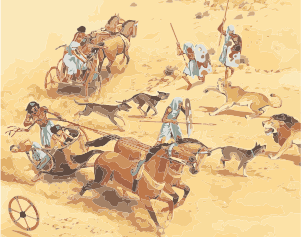
\includegraphics[width=0.48\textwidth]{pic1}
%		%		\caption{\small\textit{Hình 1}}
%		\vspace*{-10pt}
%	\end{figure}
	Ngày nay, khi muốn mua một thứ hàng hóa nào đó, chúng mình dùng tiền để mua. Nhưng ở thời xa xưa, cách đây hơn 5000 năm, con người không thể thực hiện các hoạt động mua bán bằng tiền, như ngày nay, vì ngày đó \ldots tiền chưa có! Thời đó, người ta đã dùng “trao đổi hàng hóa”, để có được những vật phẩm mà mình cần. Chuyện kể rằng, có một bộ lạc chuyên săn thú. Họ rất giỏi săn bắn, nhưng lại không giỏi trồng trọt. Thế nên, ngày qua ngày, họ không dùng hết thịt của những loại thú săn được, trong khi rất thèm ăn rau xanh. Thế là, một ngày nọ, họ đến gặp bộ lạc trồng rau và xin đổi một con thú lấy một sọt rau, quả. Bộ lạc trồng rau đồng ý. Từ đó, ngày ngày, bộ lạc săn thú mang thịt thú
	\begin{figure}[H]
		\centering
		\vspace*{-5pt}
		\captionsetup{labelformat= empty, justification=centering}
		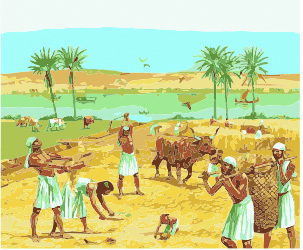
\includegraphics[width=0.47\textwidth]{pic2}
%		\caption{\small\textit{Hình 1}}
		\vspace*{-10pt}
	\end{figure}
	rừng đổi lấy rau xanh, quả ngọt của bộ lạc trồng rau. Nghe nói, có lúc, do thời tiết khắc nghiệt, rau xanh khó trồng, bộ lạc săn thú phải đổi $2$ con lợn rừng để lấy một nửa sọt rau, quả của bộ lạc trồng rau đấy.
	\vskip 0.15cm	
	Bây giờ, thỉnh thoảng bố của Bi cũng thực hiện trao đổi “hàng hóa” với Bi nha. Biết Bi thích sưu tầm ảnh của các tuyển thủ bóng đá, bố Bi đã “ra giá”, đổi một điểm $10$ lấy ảnh của ba tuyển thủ đội tuyển bóng đá U$23$ Việt Nam năm $2019$ đấy. Bố Bi còn hứa sẽ đổi một Giấy khen “Học sinh xuất sắc” lấy một năm Tạp chí Pi nhé; vì bố biết, đọc tạp chí Pi, cái phần “Toán của  mình” ấy, Bi thấy khoái quá trời khoái luôn! (Giờ, tuy Bi đang thường xuyên đọc Pi, nhưng là đọc nhờ của bố; đọc của mình thích hơn nhiều chứ, các bạn nhỉ?).
	\begin{figure}[H]
		\centering
		\vspace*{-5pt}
		\captionsetup{labelformat= empty, justification=centering}
		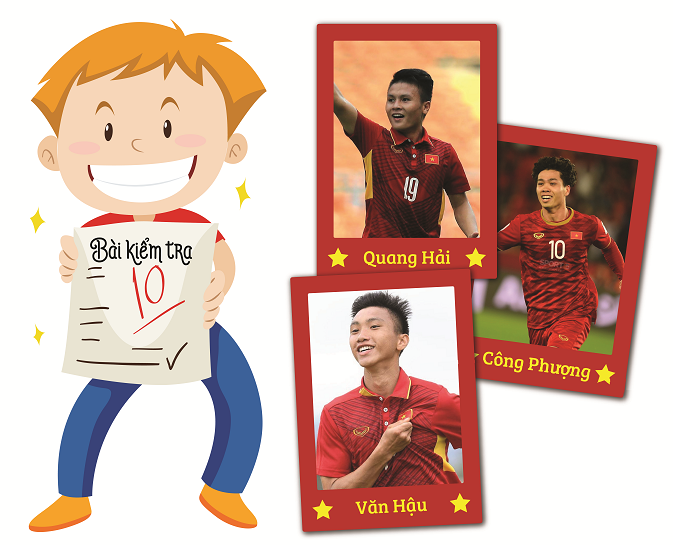
\includegraphics[width=0.47\textwidth]{pic3}
%		\caption{\small\textit{Hình 1}}
		\vspace*{-5pt}
	\end{figure}
	Tìm hiểu, Bi thấy có nhiều bài toán trao đổi hàng hóa thú vị lắm. Các bạn cùng Bi giải mấy bài toán “trao đổi” dưới đây nhé.
	\vskip 0.15cm
	\textbf{Bài toán $\pmb{1.}$} Một bộ lạc người nguyên thủy chuyên săn bắt thú. Họ đã dùng thịt thú rừng sấy khô và những tấm da thú để đổi lấy lương thực và rau, quả. Cứ $2$ đùi thịt thú rừng sấy khô sẽ đổi được $7$ sọt rau, quả; còn $21$ tấm da thú sẽ đổi được $14$ sọt rau, quả. Theo bạn, với cách đổi ấy, dùng $6$ đùi thịt thú rừng sấy khô và $9$ tấm da thú sẽ đổi được bao nhiêu sọt rau, quả?
	\vskip 0.15cm
	\textbf{Bài toán $\pmb{2.}$} Có hai quầy bán bát, đĩa, quầy $A$ và quầy $B$, nằm ở gần nhau. Với tinh thần tương thân, tương ái, chủ của hai quầy hàng đó thỏa thuận sẵn sàng trao đổi hàng hóa với nhau, trong những lúc cần hàng để phục vụ người mua. Công thức trao đổi được thống nhất là: Một bát to đổi được ba đĩa; ba bát nhỏ đổi được năm đĩa.
	\vskip 0.15cm
	Một lần, vào đúng lúc quầy $A$ vừa bán hết đĩa, có một người khách tới mua hàng, với đơn hàng như sau: Mua $12$ cái bát to, và cứ mua $3$ bát to lại mua $10$ cái bát nhỏ, cứ mua $5$ bát nhỏ lại mua $2$ cái đĩa.
	\vskip 0.15cm
	Hỏi, chủ quầy $A$ cần mang sang quầy $B$ bao nhiêu cái bát, cả to và nhỏ, để đổi được đúng số đĩa trong đơn hàng của người khách nói trên?
	\begin{figure}[H]
		\centering
		\vspace*{-5pt}
		\captionsetup{labelformat= empty, justification=centering}
		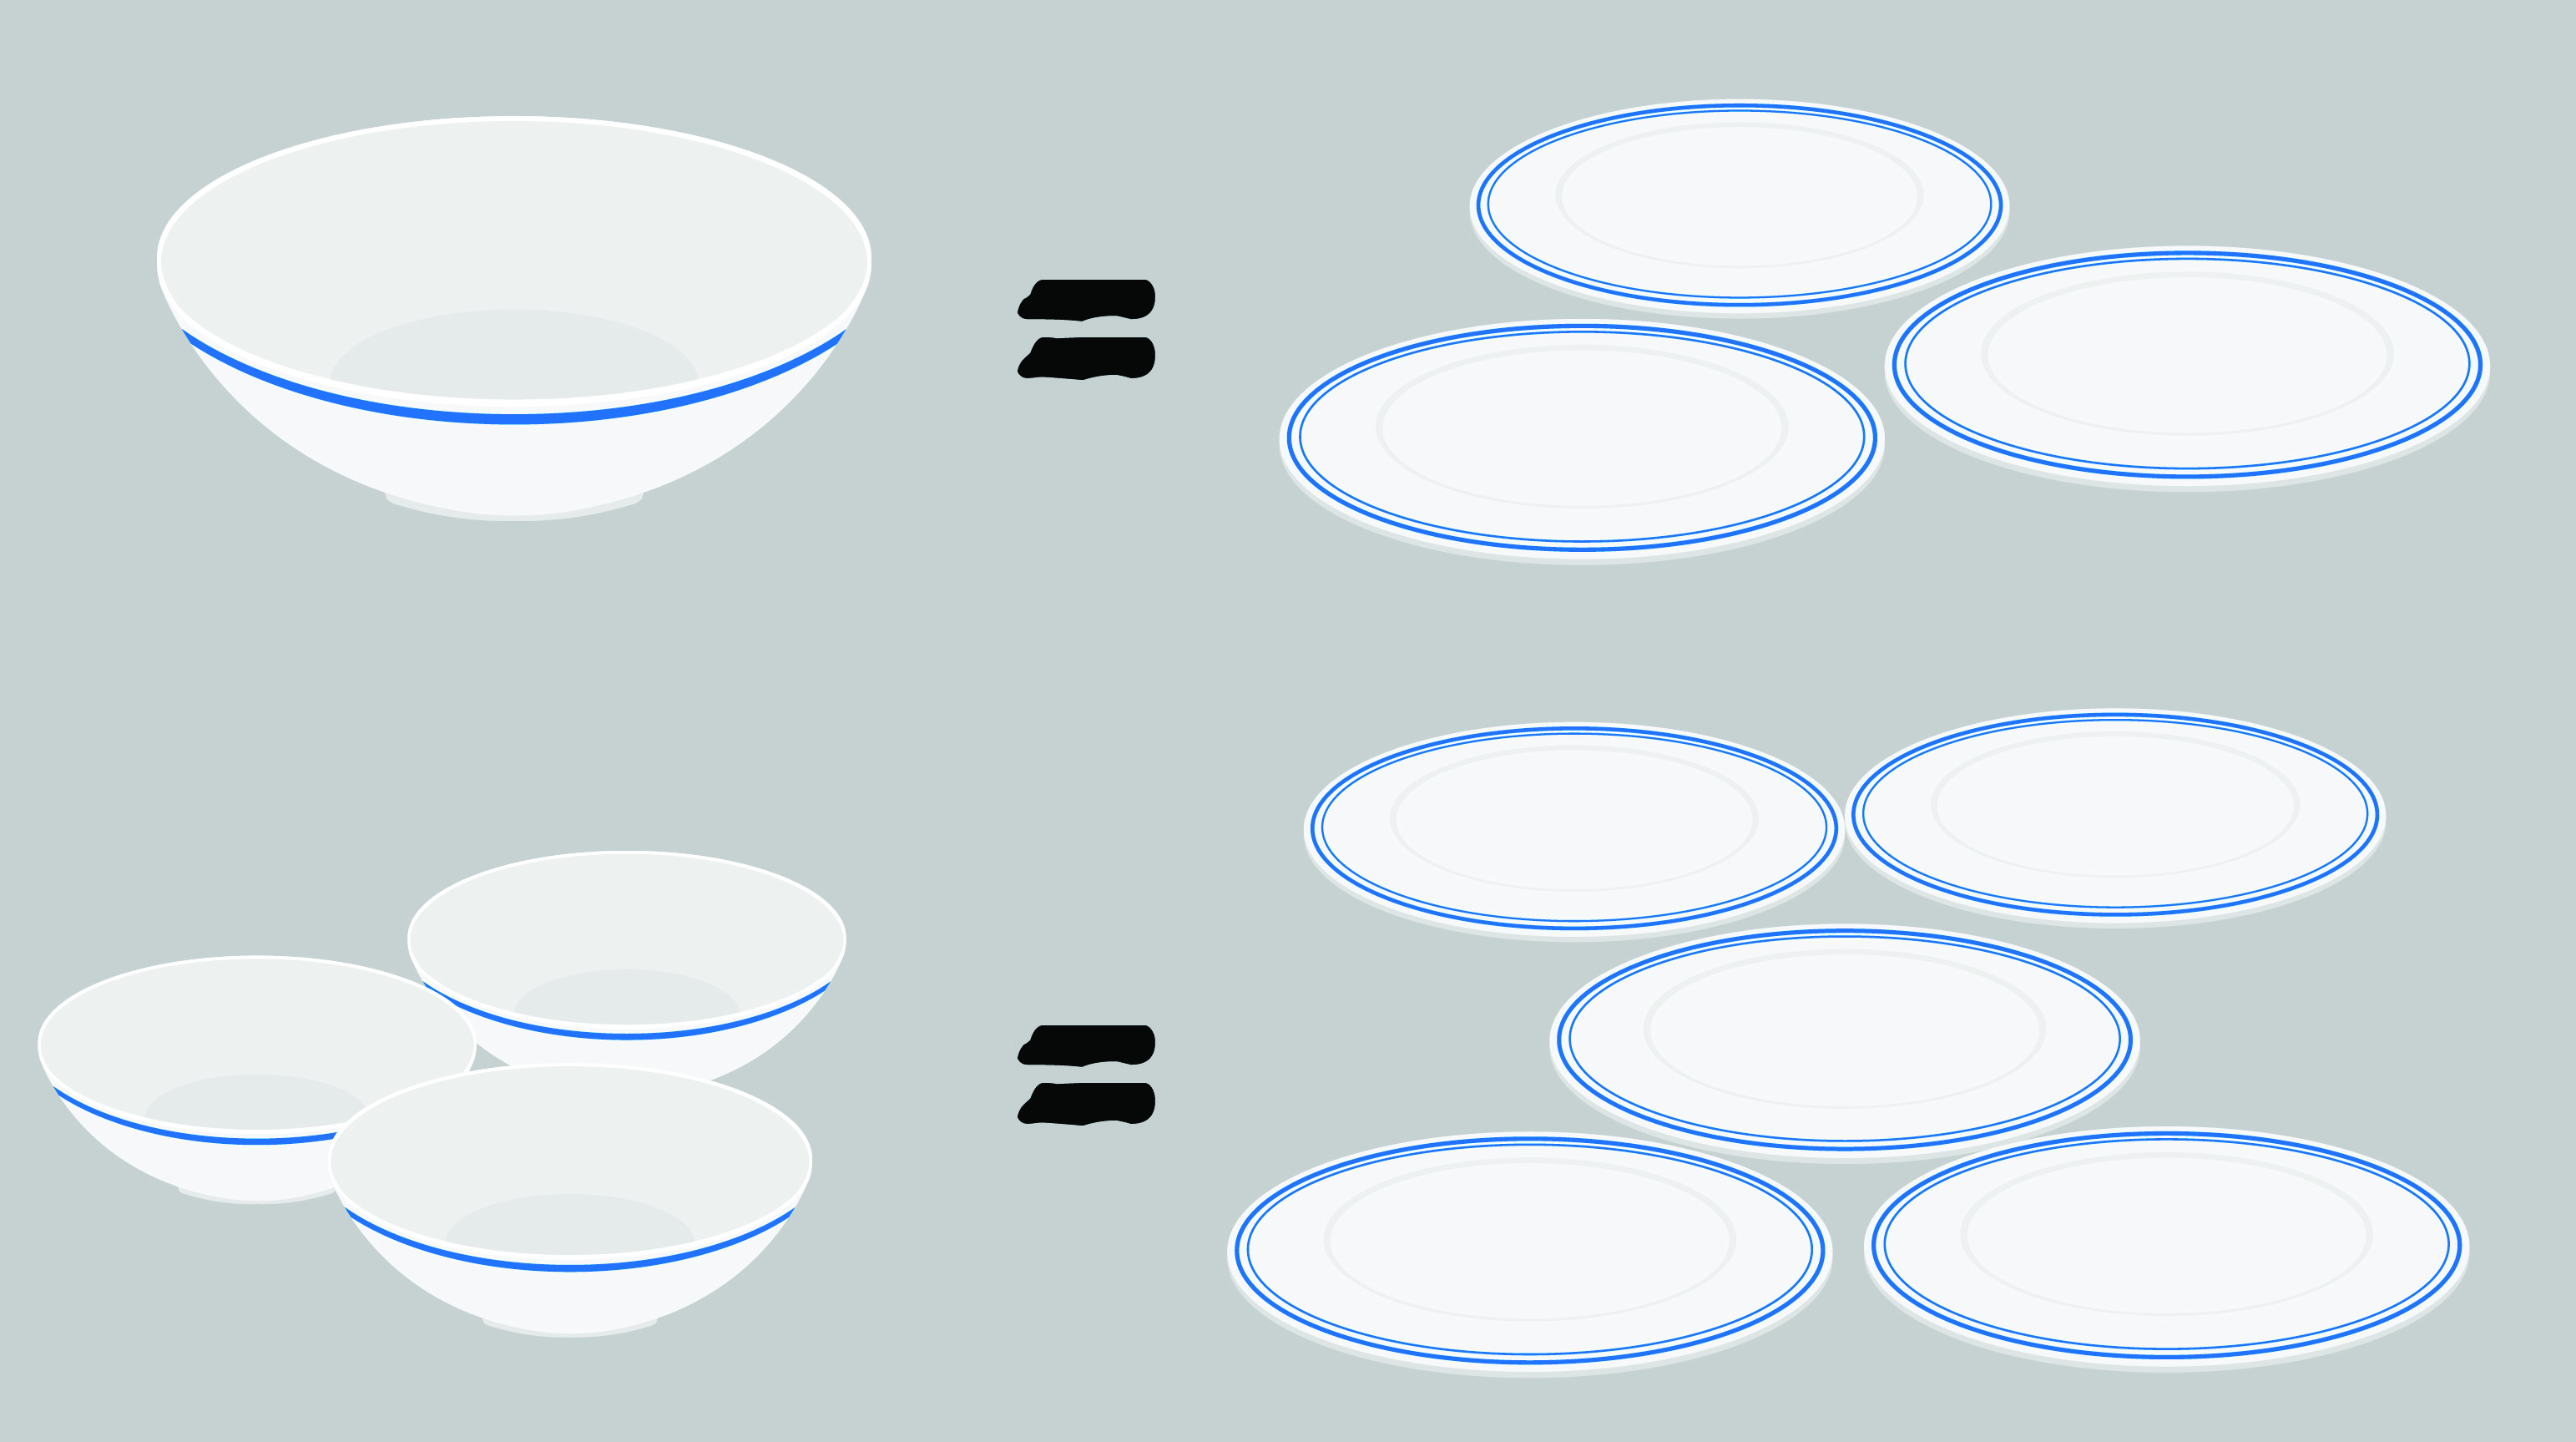
\includegraphics[width=0.47\textwidth]{pic4}
		\caption{\small\textit{Hình $1.$}}
		\vspace*{-5pt}
	\end{figure}
	\textbf{Bài toán $\pmb{3.}$} Một bác bán trứng bán bốn loại trứng, gồm trứng gà, trứng vịt, trứng ngỗng và trứng chim cút. Ngày hôm ấy, bác nhẩm ra rằng, “cứ bán được ba trứng ngỗng thì bán được năm trứng gà và bảy trứng vịt; cứ bán được năm trứng vịt thì bán được hai trứng gà và mười trứng chim cút”. Biết rằng, ngày hôm ấy, bác đã bán được $15$ quả trứng ngỗng. Hỏi bác đã bán được bao nhiêu trứng gà, bao nhiêu trứng vịt và bao nhiêu trứng chim cút, trong ngày hôm đó?
	\begin{figure}[H]
		\centering
		\vspace*{-5pt}
		\captionsetup{labelformat= empty, justification=centering}
		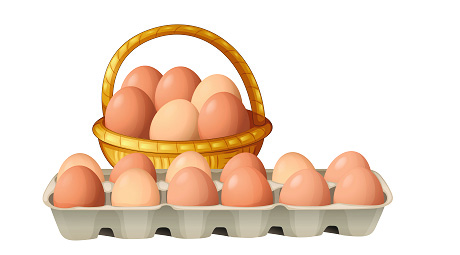
\includegraphics[width=0.53\textwidth]{pic6}
		\vspace*{-5pt}
	\end{figure}
	\textbf{Bài toán $\pmb{4.}$} Một cửa hàng bán hoa niêm yết giá bán hoa như sau:
	\vskip 0.15cm
	“Tiền mua năm bông hồng và ba bông tulip cũng bằng tiền mua một bông hồng và năm bông tulip.”
	\vskip 0.15cm
	Hỏi giá hoa nào, hồng hay tulip, đắt hơn, và đắt hơn mấy lần?
	\begin{figure}[H]
		\centering
		\vspace*{-5pt}
		\captionsetup{labelformat= empty, justification=centering}
		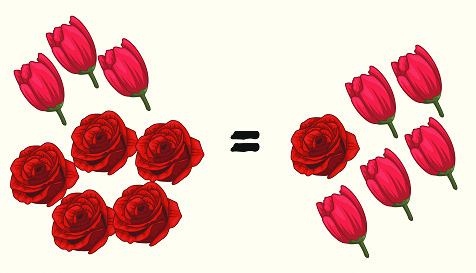
\includegraphics[width=0.47\textwidth]{pic5}
		\vspace*{-5pt}
	\end{figure}